\documentclass[12pt,a4paper]{article}
\usepackage{times}
\usepackage{durhampaper}
\usepackage{harvard}
\usepackage{amsmath}
\usepackage{tikz}
\usepackage{forest}
\usepackage{fancybox}
\usepackage{verbatim}

\citationmode{abbr}
\bibliographystyle{agsm}

\title{SAT Solvers}
\author{King Him Cheung}
\student{King Him Cheung}
\supervisor{Dr. Friedetzky}
\degree{BSc Computer Science}

\date{}
\def\layersep{2.5cm}

\begin{document}

\maketitle

\begin{abstract}\newline\newline
{\bf Context/Background}\newline \\
The purpose of SAT Solvers is the solve the satisfiability problem, they are in use in modern day technologies for many practical reasons including: model checking, hardware verification, automatic test pattern generation, planning, scheduling, and even challenging problems from algebra. Over the years, we have seen new implementations of these SAT solvers which more importantly are becoming more efficient.  
\\\\
{\bf Aims}\\\\
The aim of this project is to research modern day SAT solvers and understand the reasons to their efficiency, discovering different implementations and understanding their uses is therefore vital. Furthermore, another aim of this project and one in which concrete results can be produced is the implementation of a SAT Solver capable in solving more difficult satisfiability problems.
\\\\
{\bf Method}\\\\
Various SAT solvers should be researched, comparisons in their run times should be made and recorded. Implementation on different variations of SAT Solvers ranging from their complexity, understanding the underlying concepts of these implementations, taking into consideration the algorithm and data structures involved.   
\\\\
{\bf Proposed Solution.}\\\\
Research variations of the SAT Competition solvers as a initial look into the various implementations, compare running time of these variations, taking into account search problem implementations and other solutions.\newline
Using Python to create test implementations without consideration of advanced optimisations and then moving on to produce more optimised versions either using optimised frameworks or a more low level programming language such as C++. \newline
Research modern technologies such as machine learning and how they may be used to produce more efficient solvers.



\end{abstract}

\begin{keywords}
SAT Solver, local search problem, machine learning.
\end{keywords}
\newpage
\section{Introduction}

SAT Solvers come in many variations, this project is to understand the practical purpose of SAT Solvers, how SAT Solvers have developed over the years and how some variations are implemented. Concrete results can be gathered from comparing SAT solvers through their running times and use cases. Moreover, implementation of SAT Solvers of different variations including the use of more modern techniques will be made. Overall, this project will consider SAT Solvers from a theoretical view and implementations will be made from a theoretical approach on ideas from search problem and machine learning concepts.\\\\
{\bf Project Domain}\\\\
The boolean satisfiability problem is defined as: "does there exist a assignment of variables that satisfies the given boolean formula?" \\

In our consideration of this problem we will focus on Boolean Formulas in Conjunctive Normal Form: A conjunction of clause where a clause is the disjunctions of literals. 
\begin{itemize}
	\begin{item}
	A literal is a variable of the negation of the variable: x or $\neg$x.
	\end{item}
	\begin{item}
	A conjunction (X $\land$ Y) or (X$_1$ $\land$ X$_2$ $\land$ ... $ \land$ X$_n$) is True only when all variables are True.
	\end{item}
	\begin{item}
	A disjunction (X $\lor$ Y) or (X$_1$ $\lor$ X$_2$ $\lor$ ... $\lor$ X$_n$) is True only when at least one variable is True.
	\end{item}
\end{itemize}
This problem is NP-complete and many other problems can be encoded as a Satisfiability problem therefore by having efficient solvers for this problem means being able to solve many other problems. Some real world applications for SAT solvers include: Model checking, scheduling and problem solving.\\\\
Model Checking \cite[p. 2027]{ModelChecking} is used for hardware verification and is a technique of checking some property of the hardware by describing hardware functionality as a model: a set of states S  = $\{X_1, X_2, ..., X_n\}$ and transition relations between states  $\tau(S_1, S_2), S_1\in S$ and $S_2 \in S$. Some properties checked may include: Liveness, where a property eventually occurs e.g. used to check whether a response is eventually given or to check if cycles occur and Safety where a property always holds e.g. the reachability problem, to check whether or not a bad state can be reached. \\
Bounded model checking \cite[p. 2029]{ModelChecking} where a property is checked within some k steps can be solved by SAT solvers checking for satisfiability on the formula: \\
\begin{center}
$I(v_0) \land \bigwedge \limits_{i=0}^{k-1} \tau(v_i, v_i+1) \land \bigvee \limits_{i=0}^{k}\neg p(s_i)$ 
\end{center}
Where $I(v_0)$ is defined as $v_0$ being the initial state, and all states $v_i$ are iterated through by a legal transition state and none of the states reached have the property $p$.\\\\ 
\newpage
{\bf Project Overview}\\\\
The structure of this project will be focused on gaining insight in the multiple variations of SAT solvers from a theoretical view. Moreover, the projects goal of implementing of SAT solvers will allow a more in depth insight on workings of the algorithms.
\\\\
DPLL algorithm \cite{DPLL}- Davis Putnam Loveland Logemann - is one such variety and one that is a basis to many modern day solvers, the algorithms involves getting as input a CNF formula and outputs whether the formula is satisfiable and if it is in fact satisfiable then it returns an assignment of variables that does so. The procedure to this algorithm follows a tree where each node of the tree is a set of clauses $S$ and at each node an assignment to a variable is made. 
\begin{center}
	\begin{tikzpicture}[level/.style={sibling distance=60mm/#1}]
		\node [circle,draw] {}
			child {node [circle,draw]  {$A$}
				child {node [circle,draw]  {$B$}
					child{ node {...}}
					child{ node {...}}
					}	
				child {node [circle,draw]  {$\neg B$}
					child{ node {...}}
					child{ node {...}}
				}
			}
			child {node [circle,draw] {$\neg A$}
				child {node [circle,draw]  {}
					child{ node {...}}
					child{ node {...}}}
				child {node [circle,draw]  {}
					child{ node {...}}
					child{ node {...}}
				}
			};
	\end{tikzpicture}
\end{center}
At each node after a variable has been assigned, we then continually apply inference (propagation) and so reducing the number of assignments and thus nodes in the tree. A node no longer has children if the node has the set \{\} as its set of clauses or if the set of clauses contain the empty set $\epsilon \in$ S. \\
If a branch has \{\} has its set of clauses then the formula is satisfiable and if all branches' set of all clauses contain the empty set $\epsilon \in$ S then the formula is unsatisfiable. \\\\
CDCL \cite[p. 131]{CDCL} - Conflict Driven Clause Learning - is another variety of SAT solvers first used in Grasp \cite{GRASP} which has influenced many modern SAT Solvers, this variety of solvers is characterised by adding new clauses to its initial set of clauses as the algorithm progresses and non-chronological backtracking. As the search progresses and the branch of the search tree encounters a conflict i.e. a variable is previously set True and the most recent propagation requires the variable to be set False or vice versa. Through the conflict the algorithm learns the clause to be added to our set of clauses (clause database). The non-chronological backtracking and clause learning enables the algorithm to prune the search tree and significantly reduce the time of discovering a satisfiable assignment or to show that the formula is unsatisfiable. \\\\
There are also local search algorithms for SAT which is not complete and so may not provide an assignment of variables that satisfy the formula and may not be able to show that the formula is unsatisfiable however these algorithms can be shown to be efficient in specific cases of problems.\\
Furthermore, a more modern approach to solving SAT problems is the use of machine learning and describing the problem as a classification problem, we can classify SAT problems so that solvers more efficient on specific categories of problems can be applied, this is in contrast to the more general SAT solvers.\\\\
{\bf Project Deliverables}\\\\
{\bf Basic deliverables:}
\begin{enumerate}
		\item Implement a brute force SAT Solver using an intuitive programming language for the problem (may not be efficient)
			\begin{itemize}
				\item{- compromise on efficiency to produce a basic SAT solver using a high level language e.g. Python. Use an intuitive implementation relying on simple data structures.}
			\end{itemize}
		\item Develop understanding on a programming language that aims to increase efficiency
			\begin{itemize}
				\item{ - Read online documentation on a programming language that allows efficient use of data storage and manipulation e.g. C++, consider efficient uses of data structures and lower level data handling.}
			\end{itemize}
		\item Discover and understand optimisations made to DPLL implementations of SAT Solvers
			\begin{itemize}
				\item{-Research and develop an understanding on faster algorithms and consider the implementation of such an algorithm in the high level programming language to show proof of concept.}
			\end{itemize}
		\item Develop an understanding on machine learning
			\begin{itemize}
				\item{- Undergo an online course* on basic machine learning concepts}
			\end{itemize}	
	\end{enumerate}
{\bf Intermediate Deliverables:}
	\begin{enumerate}
		\item Research how machine learning can be applied to SAT Solving
			\begin{itemize}
				\item{- Read articles and research papers on the use of machine learning in SAT solving}
			\end{itemize}
		\item Implement a DPLL SAT Solver using an efficient programming language
			\begin{itemize}
				\item{- implement DPLL Sat Solver using the previously studied lower level programming language.}
			\end{itemize}
		\item Implement a DPLL SAT Solver involving multiple optimisations
			\begin{itemize}
				\item{- implement efficient data structures using the lower level language and implement researched optimisations to the algorithm e.g. watched literals.}
			\end{itemize}
		\item Explore and implement other versions of SAT solvers e.g. local search
	\end{enumerate}
{\bf Advanced Deliverables}
	\begin{enumerate}
		\item Analyse the efficiency benefits of the different optimisations in DPLL and its possible costs
		\item Using the knowledge of most beneficial optimisations create a SAT Solver that is as efficient as possible (with the optimisations explored)
		\item Implement a SAT Solver that utilises machine learning giving its benefits and costs
	\end{enumerate}

%overview -
% - Describe Satisfiability Problem
% - Describe problem as a solution of a search problem
% - Describe the variations of this problem

%Project Purpose - 
% - Learn theoretical concepts
% - Implement an intermediate SAT Solver
% - research modern SAT Solver variations 

% Deliverables
% Use deliverables found in Literature Review


%This section briefly introduces the project, the research question you are addressing.  Do not change the font sizes or line spacing in order to put in more text.

%Note that the whole report, including the references, should not be longer than 12 pages in length (there is no penalty for short papers if the required content is included). There should be at least 5 referenced papers.

%Programming Language
%Python (ease of programming and fast implementation) and C++ (mid level language allows for low level control and so more optimal implementation)

%Algorithms
%Pseudocode and explanation of different algorithms
%DPLL
%CDCL
%Grasp/zChaff
%Competition Examples
%Neural Nets?
%logical Regression 
%Local Search Sat Solvers

%Testing 
%Unit Testing
%Comparison of algorithms
%Run against multiple examples and check speed

\section{Design}
The design outcome of this project is to produce multiple SAT solvers that can take as input a text file of the satisfiability problem in DIMACS format  \cite{dimacsFormat}[http://www.domagoj-babic.com/uploads/ResearchProjects/Spear/dimacs-cnf.pdf] \\\\
\texttt{
c - this is a comment\\
c \\
c \\
p cnf 5 3\\
1 -5 4 0\\
-1 5 3 4 0\\
-3 -4 0\\
}\\
Where lines beginning with c is a comment, the line beginning with p is the format of the file e.g. the above file "p cnf 5 3" is in Conjunctive Normal Form (CNF), has 5 variables and 3 clauses. The lines below the one starting with p are the clauses of the satisfiability problem where each number denotes the variable and a minus symbol denotes the variables negation. The end of the clause is also represented by a 0.\\\\

{\bf Choice of Programming Language} \\\\
The two languages utilised in this project will be python and C++, I have used Python throughout my undergraduate studies giving me a firm familiarity with Python and therefore understanding its ease of implementation however lack of low level options resulting in less than optimal [programs]. \\
The high level nature of Python allows for fast proof of concept of algorithms allowing me test and run to different implementations quickly. This will be valuable as there are many variations of SAT solvers and a large portion of this project is to research algorithms in comparison to solely implementing them. \\
Morever, there are multiple machine learning libraries for Python and so in combination with Python's high level nature will provide a suitable level of support for testing machine learning concepts, one such example of these libraries is Pytorch a popular machine learning library and so will also result in external support such as tutorials. \\
On the other hand, C++ is a middle level language allowing for lower level control which will prove useful when producing more optimal implementations with the focus on reducing run time.\\
As we will comparing run times of implementations it will be useful to remove overheads provided from the language and so C++ is a more suitable language for this purpose. \\\\

{\bf SAT Solver Variations}\\\\
{\bf DPLL}\\
The DPLL algorithm is a backtracking search of possible assignments of variables.Our implementation of this algorithm will follow the simplest depth first search version, a recursive form \cite[p. 92]{DPLL-Implementation} that branches on a decided variable.\\
We initially run unit propagation on our input clauses and check for satisfiability or unsatisfiability. Unit propagation is the search for any unit clauses, where a unit clause is a clause that contains only one literal, after finding a unit clause we then fix the literal (i.e. a variable or its negation) found in the unit clause to True, furthermore, for every clause that contains the literal we remove from our set of clauses as well as removing negations of literals from all clauses.\\
We then check for an empty set of clause to indicate that the problem is satisfied, whereas if there is an empty set within our set of clause then the problem is unsatisfied.\\ 
After the initial check for satisfiability and unsatisfiability we then decide a variable to branch on, the function is recursively called twice on the set of clauses with the addition of either adding a unit clause of the variable in one case or a unit clause of it's negation in the other case.
\texttt{
\begin{center}Unit Propagation \end{center} 
Input Boolean Formula:\\ \hspace*{1cm} (p $\lor$ q  $\lor$ r) $\land$ ($\neg$p $\lor$ r) $\land$ (p $\lor$ s) \\
Decide:\\ \hspace*{1cm} Set literal  to true e.g. assign $\neg$p to True. \\
Update clauses:\\ \hspace*{1cm} (q $\lor$ r) $\land$ (s)\\
Find Unit Clauses:\\ \hspace*{1cm}  (q $\lor$ r) $\land$ \textbf{(s)} \\
Unit Propagation:\\ \hspace*{1cm} Set literal in unit clause to true e.g. assign s to True.
}\\\\
Resolve - Once all assignments have been propagated and there are no longer any new variables to be assigned a value we check to see if there are any conflicts. If a conflict exists we backtrack, in our basic variafhtion of our DPLL algorithm we backtrack to the last decision stage in which both values has not yet been assigned to the variable.\\\\
\texttt{
Input : A CNF formula F and an initially empty partial assignment $\rho$ \\
Output : UNSAT, or an assignment satisfying $F$\\
begin\\
\hspace*{1cm}$(F,\rho)$ $\leftarrow$ UnitPropagate $(F,\rho)$\\
\hspace*{1cm}if $F$ contains the empty clause then return UNSAT\\
\hspace*{1cm}if $F$ has no clauses left then Output $\rho$ return SAT\\
\hspace*{1cm}$l \leftarrow$ a literal not assigned by $\rho$  //the branching step \\
\hspace*{1cm}if DPLL-recursive $(F |_\ell,\rho \cup \{\ell\})$ = SAT then return SAT\\
\hspace*{1cm}return DPLL-recursive$(F |_{\neg\ell},\rho \cup \{\neg l \})$ \\
end
}
\begin{center}Pseudocode for DPLL Implementation \cite[p. 93]{DPLL-Implementation} \end{center}
The DPLL is an early SAT Solver and our implementation has many optimisations that can be added, for example we can consider: 
\begin{itemize}
	\item{More optimally deciding which variable to branch on.}
	\item{Ignoring branches that will not have a satisfying assignment.}
\end{itemize}
\hfill\\
{\bf CDCL}\\
CDCL Solvers are a variation of the DPLL algorithm and employs clause learning and other optimisations. Clause learning is the addition of learnt clauses to the original boolean formula throughout the running of the algorithm and is what distinguishes a CDCL solver to the original DPLL solvers. Our CDCL implementation will follow a repeating three stage process: Decide, Deduce and Resolve. 
\begin{enumerate}
	\item{Decide - At the decide stage of our algorithm we select a variable and assign it a value 0 or 1.}
	\item{Deduce - After the decide stage, remove all clauses with literals of which evaluates to True due to the decided variable assignment, moreover, remove all literals from clauses where that literal evaluates to false after the decided variable. Finally, we can see if we can deduce any new assignment of variables through unit propagation.}
	\item{Resolve - Once all assignments have been propagated and there are no longer any new variables to be assigned a value we check to see if there are any conflicts. If a conflict exists we backtrack to the first unique implication point (UIP), from the conflict we can also learn new clauses that can be added to our input set of clauses.}
\end{enumerate}
\texttt{CDCL$(\phi, v)$
\begin{enumerate}
\itemsep0em
\item{
if (UnitPropagation$(\phi, v)$ == CONFLICT) }
\item{
\hspace*{0.5 cm} then return UNSAT}
\item{
dl $\leftarrow$ 0}
\item{
while (not AllVariablesAssigned$(\phi, v))$}
\item{
\hspace*{0.5cm} do $(x, v)$ = PickBranchingVariable$(\phi, v)$ \bf{[decide stage]}} 
\item{
\hspace*{1cm} $dl \leftarrow dl + 1$}
\item{
\hspace*{1.5cm} $v \leftarrow v \cup \{ (x, v) \}$}
\item{
\hspace*{2cm}if (UnitPropagation$(\phi, v)$ == CONFLICT) \bf{[deduce stage]}}
\item{
\hspace*{2.5cm} return SAT}
\item{
\hspace*{3cm} then $\beta$ = ConflictAnalysis$(\phi, v)$ if $(\beta < 0)$ \bf{[resolve stage]}}
\item{
\hspace*{3.5cm} then return UNSAT }
\item{
\hspace*{3.5cm} else Backtrack$(\phi, v, \beta)$}
\item{
\hspace*{4cm} $dl \leftarrow \beta$ }
\end{enumerate}
}
\begin{center}Pseudocode for CDCL Implementation \cite[p. 136]{CDCL} \end{center}
Definitions \cite[p.132]{CDCL}:\\
\begin{itemize}
\item{
Decision Level: every literal has a decision level $\delta(l)$, at each decision stage of our algorithm the decision level is incremented and the decided literal is set the new decision level, during the unit propagation stage if a literal is fixed True then its decision level is set the same as the decision level of the most recent decided literal.}
\item{
Antecedent: Every variable has a antecedent $\alpha(l)$, this is the original clause of the unit clause during unit propagation stage that caused the assignment of the variable. Variables assigned at the decide stage is set the empty clause as its antecedent.}
\item{
A predicate $\xi$ that returns True if a clause has a literal that has a decision level equal to the current decision level and if that literal is implied from a unit clause i.e. has antecedent that is not NIL.
\[ \xi(\omega, l, d) =
  \begin{cases}
    True & \quad \text{if } l \in \omega \land \delta(l) = d \land \alpha(l) \neq  NIL\\
    False & \quad \text{otherwise }
  \end{cases}
\]

}
\item{
A function $\sigma$ that takes input a clause $\omega$ and a decision level $\delta$ and returns the number of literals in a clause that has literal equal to the input decision level.
\[\sigma(\omega, d) = |{l \in \omega | \delta(l) = d }| 
\]
}
\end{itemize}
In this project I will focus only a few of the many optimisations for CDCL including: clause learning with UIP (unique implication points), lazy data structures with watched literals and backtracking to the first UIP.
\begin{enumerate}
\item{clause learning with UIP \cite{GRASP} - Conflicts occur during the unit propagation stage, we search through the antecedents of variables of the highest decision level, those that were assigned during the most recent unit propagation, from these antecedents we add to a empty clause the literals that have a decision level value lower than the current decision level, finding such variables is achievable through resolution, this new clause will be the learnt clause and is added to our current set of clauses.\\\\
\texttt{
Resolution$(\omega1, \omega2)$ or more simply $\omega1\odot\omega2$: \\
Input: two clauses with one containing unique variable x and the other containing $\neg$x :\\ \hspace*{1cm} $\omega1$ = (x $\lor$ y1  $\lor$ y2 $\lor$ ...), $\omega2$ = ($\neg$x $\lor$ z1 $\lor$ z2 $\lor$ ...)\\\\
Output: clause containing all variables found in both clauses except x and $\neg$x:\\ \hspace*{2.5cm} (y1  $\lor$ y2 $\lor$ ... $\lor$ z1 $\lor$ z2 $\lor$ ...)
}\\\\
Using resolution and our definitions we can now produce a method of finding a learnt clause after a conflict, this method uses the first unique implication point, i.e. when the number of literals that has equal decision level to the current decision level is equal to 1:\\
\[ \omega_L ^{d, i} = 
  \begin{cases}
    \alpha(\kappa) & \quad \text{if } i = 0\\
    \omega_L ^{d, i-1} \odot \alpha(l) & \quad \text{if } i \neq 0 \land \xi(\omega_L ^{d, i-1}, l, d) = 1\\
     \omega_L ^{d, i-1} & \quad \text{if } i \neq 0 \land \sigma(\omega_L ^{d, i-1}, d) = 1
  \end{cases}
\]
Where $\kappa$ is the conflict clause.
}
\item{Watched Literals \cite{chaff}- This is a lazy data structure, it's implementation is to use references to two literals of each clause in our input set of clauses, simply by referencing only two variables we do not need to scan every literal in our clause to test for a unit clause instead we update our reference to another literal if the watched literal is fixed False, whereas if a watched literal is fixed True then the references to the watched literals no longer need updating as the entire clause is satisfied. At the point where one watched literal is fixed false and the other can not reference any another literals left in the clause of which its variable has not been assigned then the clause is a unit clause.\\
\begin{center}
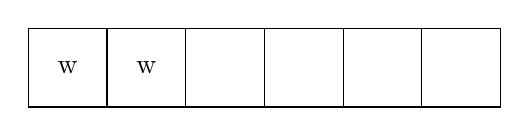
\begin{tikzpicture}
\draw (0,0) -- (1,0) -- (1,1) -- (0,1) -- (0,0) node at (0.5, 0.5){w};
\draw (1,0) -- (2,0) -- (2,1) -- (1,1) -- (1,0) node at (1.5, 0.5){w};
\draw (2,0) -- (3,0) -- (3,1) -- (2,1) -- (2,0);
\draw (3,0) -- (4,0) -- (4,1) -- (3,1) -- (3,0);
\draw (4,0) -- (5,0) -- (5,1) -- (4,1) -- (4,0);
\draw (5,0) -- (6,0) -- (6,1) -- (5,1) -- (5,0);
\end{tikzpicture}\\
\end{center}
Clause represented by array - first two literals are watched literals.\\
\begin{center}
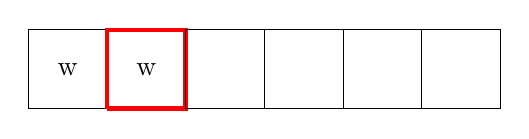
\begin{tikzpicture}
\draw (0,0) -- (1,0) -- (1,1) -- (0,1) -- (0,0) node at (0.5, 0.5){w};
\draw [red, ultra thick](1,0) -- (2,0) -- (2,1) -- (1,1) -- (1,0) node [black] at (1.5, 0.5){w};
\draw (2,0) -- (3,0) -- (3,1) -- (2,1) -- (2,0);
\draw (3,0) -- (4,0) -- (4,1) -- (3,1) -- (3,0);
\draw (4,0) -- (5,0) -- (5,1) -- (4,1) -- (4,0);
\draw (5,0) -- (6,0) -- (6,1) -- (5,1) -- (5,0);
\end{tikzpicture}\\
\end{center}
Second literal fixed to False.
\begin{center}
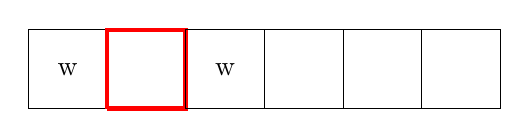
\begin{tikzpicture}
\draw (0,0) -- (1,0) -- (1,1) -- (0,1) -- (0,0) node at (0.5, 0.5){w};
\draw [red, ultra thick](1,0) -- (2,0) -- (2,1) -- (1,1) -- (1,0);
\draw (2,0) -- (3,0) -- (3,1) -- (2,1) -- (2,0) node at (2.5, 0.5){w};
\draw (3,0) -- (4,0) -- (4,1) -- (3,1) -- (3,0);
\draw (4,0) -- (5,0) -- (5,1) -- (4,1) -- (4,0);
\draw (5,0) -- (6,0) -- (6,1) -- (5,1) -- (5,0);
\end{tikzpicture}\\
\end{center}
Second watched literals reference is set to another literal that has not yet been fixed.
\begin{center}
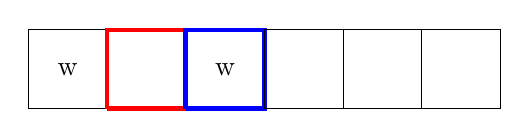
\begin{tikzpicture}
\draw (0,0) -- (1,0) -- (1,1) -- (0,1) -- (0,0) node at (0.5, 0.5){w};
\draw [red, ultra thick](1,0) -- (2,0) -- (2,1) -- (1,1) -- (1,0);
\draw [blue, ultra thick](2,0) -- (3,0) -- (3,1) -- (2,1) -- (2,0) node [black] at (2.5, 0.5){w};
\draw (3,0) -- (4,0) -- (4,1) -- (3,1) -- (3,0);
\draw (4,0) -- (5,0) -- (5,1) -- (4,1) -- (4,0);
\draw (5,0) -- (6,0) -- (6,1) -- (5,1) -- (5,0);
\end{tikzpicture}\\
\end{center}
One watched literal is fixed True so watched literals no longer need updating.
\begin{center}
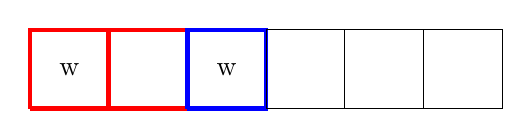
\begin{tikzpicture}
\draw [red, ultra thick](0,0) -- (1,0) -- (1,1) -- (0,1) -- (0,0) node [black] at (0.5, 0.5){w};
\draw [red, ultra thick](1,0) -- (2,0) -- (2,1) -- (1,1) -- (1,0);
\draw [blue, ultra thick](2,0) -- (3,0) -- (3,1) -- (2,1) -- (2,0) node [black] at (2.5, 0.5){w};
\draw (3,0) -- (4,0) -- (4,1) -- (3,1) -- (3,0);
\draw (4,0) -- (5,0) -- (5,1) -- (4,1) -- (4,0);
\draw (5,0) -- (6,0) -- (6,1) -- (5,1) -- (5,0);
\end{tikzpicture}\\
\end{center}
}
\item{Backtracking to first UIP \cite{firstUIPbacktrack} - Simply this means that a backtrack level is set to highest decision level in the learnt clause and the current decision level is set to the backtrack level, moreover, all literals whose decision level is greater than or equal to the backtrack level is unfixed and their antecedents reset.}

\end{enumerate}
\newpage
{\bf Local Search Algorithms}\\\\
A local search algorithm can be described by a search space in which the algorithm traverses through going along a transition from one state to another (a state is a candidate answer to our search problem) if there is a local transformation of that state to the next, each state has a calculated value which in our traversal of this space we want to maximise.
Local search algorithms are used to solve optimisation problems in contrast to our satisfiability problem which a decision problem, therefore we can translate our satisfiability problem to a suitable optimisation problem: MAX-SAT.\\\\
MAX-SAT: Find a assignment of variables that satisfies the maximum number of clauses when given as input a boolean formula in context normal form.\\\\
The algorithm we will look at in this project will be Walksat \cite{WalkSat} which we will implement as a incomplete algorithm to solve our satisfiability problem.\\
Walksat is a variation of GSAT, where GSAT is an algorithm that simply starts with a random assignment of variables and for set number of a tries MAX-TRIES it flips a set number of variables MAX-FLIPS, each flip is decided if it results in the greatest decrease in the number of unsatisfied clauses.\\
Walksat is a slight variation of GSAT: it also starts with a random assignment of variables but then instead randomly selects a unsatisfied clause and either randomly or greedily selects a variable to flip. The maximum number of flips each iteration is again defined by MAX-FLIP and the maximum number of iterations is MAX-TRIES.\\\\
\texttt{
WALKSAT($\phi, v$):
\begin{enumerate}
\item{
\hspace*{0.5cm}for i $\leftarrow$ 1 to MAX TRIES}
\item{
\hspace*{1cm}$v \leftarrow$ a random assignment of all variables
}
\item{
\hspace*{1cm}for j $\leftarrow$ 1 to MAX FLIPS}
\item{
\hspace*{1.5cm}if $v$ satisfies $\phi$ then return $v$
}
\item{
\hspace*{1.5cm} Randomly select an unsatisfied clause and flip any\\\hspace*{1.5cm} variable inside the clause that results in greatest \\\hspace*{1.5cm} decrease (can be 0 or negative) in the number of \\\hspace*{1.5cm} unsatisfied clauses}
\item{
\hspace*{1cm}end for}
\item{
\hspace*{0.5cm}end for}
\item{
return UNSAT}
\end{enumerate}
}\hfill\\
{\bf SAT Solvers with Machine Learning}\\
More modern day SAT solvers are now implementing machine learning techniques, however these solvers act differently to our previous variations instead of solving a satisfiability problem they instead classify a problem to one of the solvers in a small list of SAT solvers in what is called a SAT solver portfolio \cite{satzilla}, by classifying a SAT problem to one of many solvers the intent is to select the fastest solver for that specific problem. \\\\
Due to the time restraint of this project I will not be implementing my own SAT solver portfolio and will instead focus on the machine learning techniques instead. In this project we will attempt to apply neural networks to classify SAT problems, in order to this we must consider features most suitable for the network to learn from such that there is enough variety so there isn't under-fitting, furthermore each feature should contribute to the network and not be redundant. \\\\ 
Some features \cite{machineLearningFeatures} to consider may include: Number of clauses, number of variables, number of clauses of specific size, time required to create clause graph, time required to create variable graph and many more.\\\\
Neural networks consist of "neurones" in our case these will be logistic units, the input layer these logistic units will output the features calculated from the example sat problem, from this every input neurone is connected to a neurone in the next hidden layer and we can calculate values using a logistic function values in what is known as forward propagation and it is with this forward propagation we can classify our problem.\\\\
However, for this classification to be more accurate we must optimise the "neurones" within the network by running back-propagation, this will result in gradient descent of the squared error cost function of our predicted classification.\\\\
\begin{center}
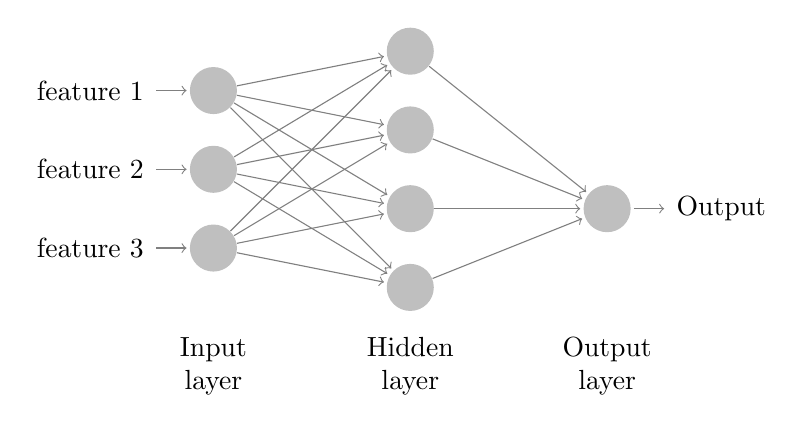
\begin{tikzpicture}[shorten >=1pt,->,draw=black!50, node distance=\layersep]
    \tikzstyle{every pin edge}=[<-,shorten <=1pt]
    \tikzstyle{neuron}=[circle,fill=black!25,minimum size=17pt,inner sep=0pt]
    \tikzstyle{input neuron}=[neuron];
    \tikzstyle{output neuron}=[neuron];
    \tikzstyle{hidden neuron}=[neuron];
    \tikzstyle{annot} = [text width=4em, text centered]

    % Draw the input layer nodes
    \foreach \name / \y in {1,...,3}
    % This is the same as writing \foreach \name / \y in {1/1,2/2,3/3,4/4}
        \node[input neuron, pin=left:feature \y] (I-\name) at (0,-\y) {};

    % Draw the hidden layer nodes
    \foreach \name / \y in {1,...,4}
        \path[yshift=0.5cm]
            node[hidden neuron] (H-\name) at (\layersep,-\y cm) {};

    % Draw the output layer node
    \node[output neuron,pin={[pin edge={->}]right:Output}, right of=H-3] (O) {};

    % Connect every node in the input layer with every node in the
    % hidden layer.
    \foreach \source in {1,...,3}
        \foreach \dest in {1,...,4}
            \path (I-\source) edge (H-\dest);

    % Connect every node in the hidden layer with the output layer
    \foreach \source in {1,...,4}
        \path (H-\source) edge (O);

    % Annotate the layers
    \node[annot,below of=H-4, node distance=1cm] (hl) {Hidden layer};
    \node[annot,left of=hl] {Input layer};
    \node[annot,right of=hl] {Output layer};
\end{tikzpicture}
\end{center}
{\bf Testing and Evaluation}\\
In order to evaluate the variety of SAT solvers that will be produced in this project we will use example sat problems that has been provided as a resource for the sat competitions, these examples are found in the sat competition website \cite{satComp} and are categorised in whether the problem is satisfiable or not and also gives a variety of sat problems in terms of number of clauses and variables and overall structure of variables found in the clauses.\\
With this data we can test given a standard amount of time e.g. 6000 seconds on average what is the highest number of variables can a specific solver take as input and still be able to provide an assignment of variables, therefore we can acquire a comparison on the overall performance of SAT solvers. \\
Moreover, we will evaluate individually how optimisations can affect the performance of solvers and whether optimisations or variations of solvers work well on every instance of the sat problem or specific cases.





\bibliography{projectpaper}


\end{document}